\chapter{F�ggel�k}

\section{A Nintendo Game Boy hivatalos architekt�r�ja}
\begin{figure}[ht]
    \centering
    \includegraphics[width=\textwidth-3.2cm, trim={0 6cm 0 0},clip]{./Resources/v2/eps/GBarchpatent.eps}
    \caption{\textit{A szabadalomban szerepl� Game Boy architekt�ra}}
    \label{fig:architecture}
\end{figure}

\section{A processzor opk�d t�bl�i}

\begin{figure}[h!]
    \centering
    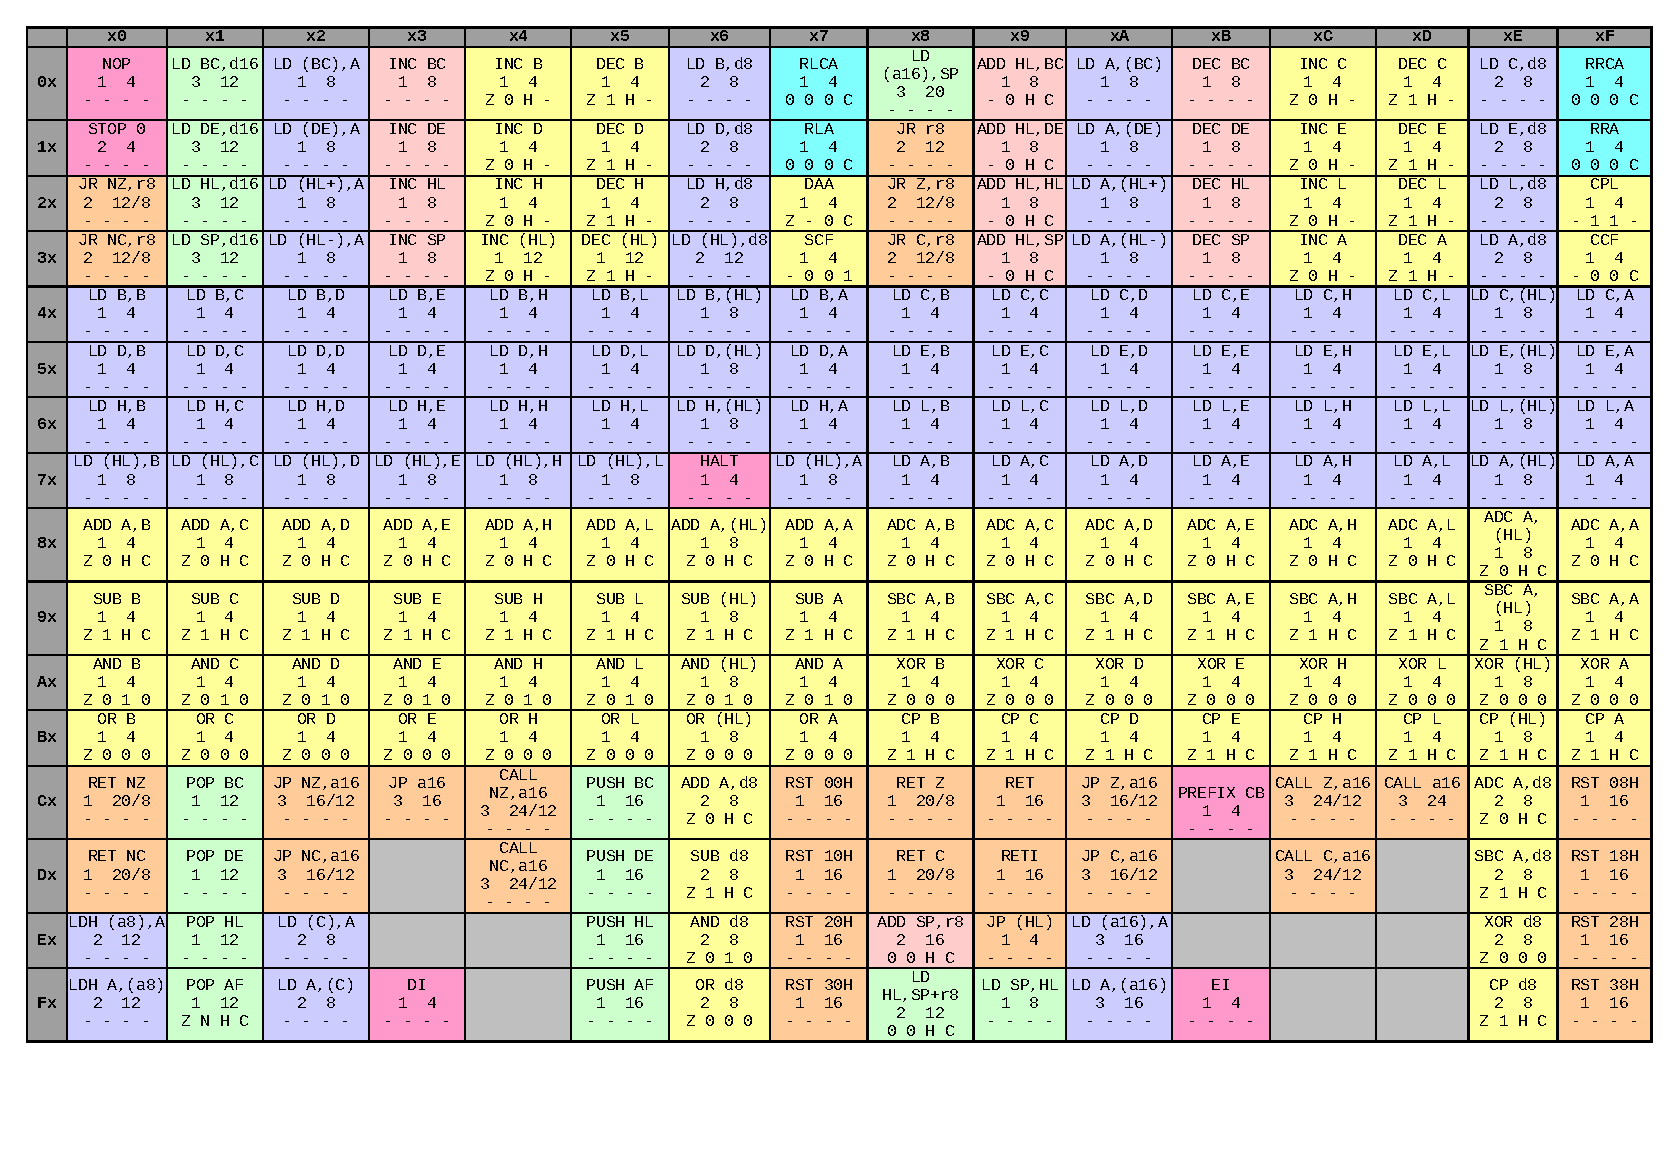
\includegraphics[height=\textheight-10.25cm,angle=-90,origin=c,trim={0 1.5cm 0 0},clip]{./Resources/Appendix/opcodes_2.eps}
    \caption{\textit{Az els� 256 opk�dot tartalmaz� t�bla}}
    \label{fig:opcodes}
\end{figure}

\begin{figure}[h!]
    \centering
    \includegraphics[height=\textheight-10.2cm,angle=-90,origin=c,trim={0 3cm 0 0},clip]{./Resources/Appendix/opcodes_cb_2.eps}
    \caption{\textit{A m�sodik, CB prefix� 256 opk�dot tartalmaz� t�bla}}
    \label{fig:opcodescb}
\end{figure}